\documentclass[handout,nooutcomes]{ximera}
\usepackage{booktabs}
%% handout
%% space
%% newpage
%% numbers
%% nooutcomes

\renewcommand{\outcome}[1]{\marginpar{\null\vspace{2ex}\scriptsize\framebox{\parbox{0.75in}{\begin{raggedright}P\arabic{problem} Outcome: #1\end{raggedright}}}}}

\renewenvironment{freeResponse}{
\ifhandout\setbox0\vbox\bgroup\else
\begin{trivlist}\item[\hskip \labelsep\bfseries Solution:\hspace{2ex}]
\fi}
{\ifhandout\egroup\else
\end{trivlist}
\fi}

\newcommand{\RR}{\mathbb R}
\renewcommand{\d}{\,d}
\newcommand{\dd}[2][]{\frac{d #1}{d #2}}
\renewcommand{\l}{\ell}
\newcommand{\ddx}{\frac{d}{dx}}
\everymath{\displaystyle}
\newcommand{\dfn}{\textbf}
\newcommand{\eval}[1]{\bigg[ #1 \bigg]}


\title{Breakout Session 8: Working with derivatives}  

\begin{document}
\begin{abstract}
  \textbf{A look back:} In the previous (February 2, 2016) Breakout Session you were introduced to the concept of the derivative of a function and the connection between derivatives and slopes of tangent lines.

  \textbf{Overview:} In today's (February 4, 2016) Breakout Session you will  study the connection between the graph of a function and the graph of its derivative.

  \textbf{A look ahead:} In the next (February 9, 2016) Breakout Session you will practice the basic rules of differentiation.
  These rules will help us to quickly compute derivatives.
  Becoming comfortable and proficient with computing derivatives is an important skill to practice before we return our focus on the conceptual aspects (and interpretation) of derivatives. 
\end{abstract}
\maketitle

\section{Learning Outcomes}
\label{section:learning-outcomes}
The following outcomes are \emph{not an exhaustive} list of the skills you will need to develop and integrate for demonstration on quizzes and exams.
This list is meant to be a starting point for conversation (with your Lecturer, Breakout Session Instructor, and fellow learners) for organizing your knowledge and monitoring the development of your skills.
\begin{itemize}
  \item 
    Estimate the slope of the tangent line graphically. 

  \item 
    Graph the derivative function.

  \item 
    Determine whether a piecewise function is differentiable.

  \item 
    Understand the relationship between the graph of a function and the graph of its derivative.

  \item 
    Understand the relationship between differentiability and continuity.
\end{itemize}

\newpage
\begin{problem}
  \mbox{}
  \begin{itemize}
    \item[(I)]
      If $f'(2)$ exists, then
      \begin{itemize}
        \item[(a)]
          $\lim_{x \to 2} f(x)$ must exist, but more information is needed if we want to find it.

        \item[(b)]
          $\lim_{x \to 2} f(x) = f(2)$.

        \item[(c)]
          $\lim_{x \to 2} f(x) = f'(2)$

        \item[(d)] 
          $\lim_{x \to 2} f(x)$ need not exist.
      \end{itemize}

    \item[(II)]
      Assuming that $\lim_{x \to 0} \frac{\sin x}{x} = 1$, we can conclude
      \begin{itemize}
        \item[(a)]
          $\frac{0}{0} = 1$
        \item[(b)]
          the tangent line to $y = \sin x$ at $(0,0)$ has slope $1$.

        \item[(c)]
          you can cancel the $x$'s.

        \item[(d)]
          for all $x$ near $0$, $\sin x = x$.

        \item[(e)]
          for all $x$ near $0$, $\sin x \approx x$.
      \end{itemize}
  \end{itemize}
\end{problem}

\begin{problem}
  Suppose we are given the graph of a function $f$:
  \begin{image}
    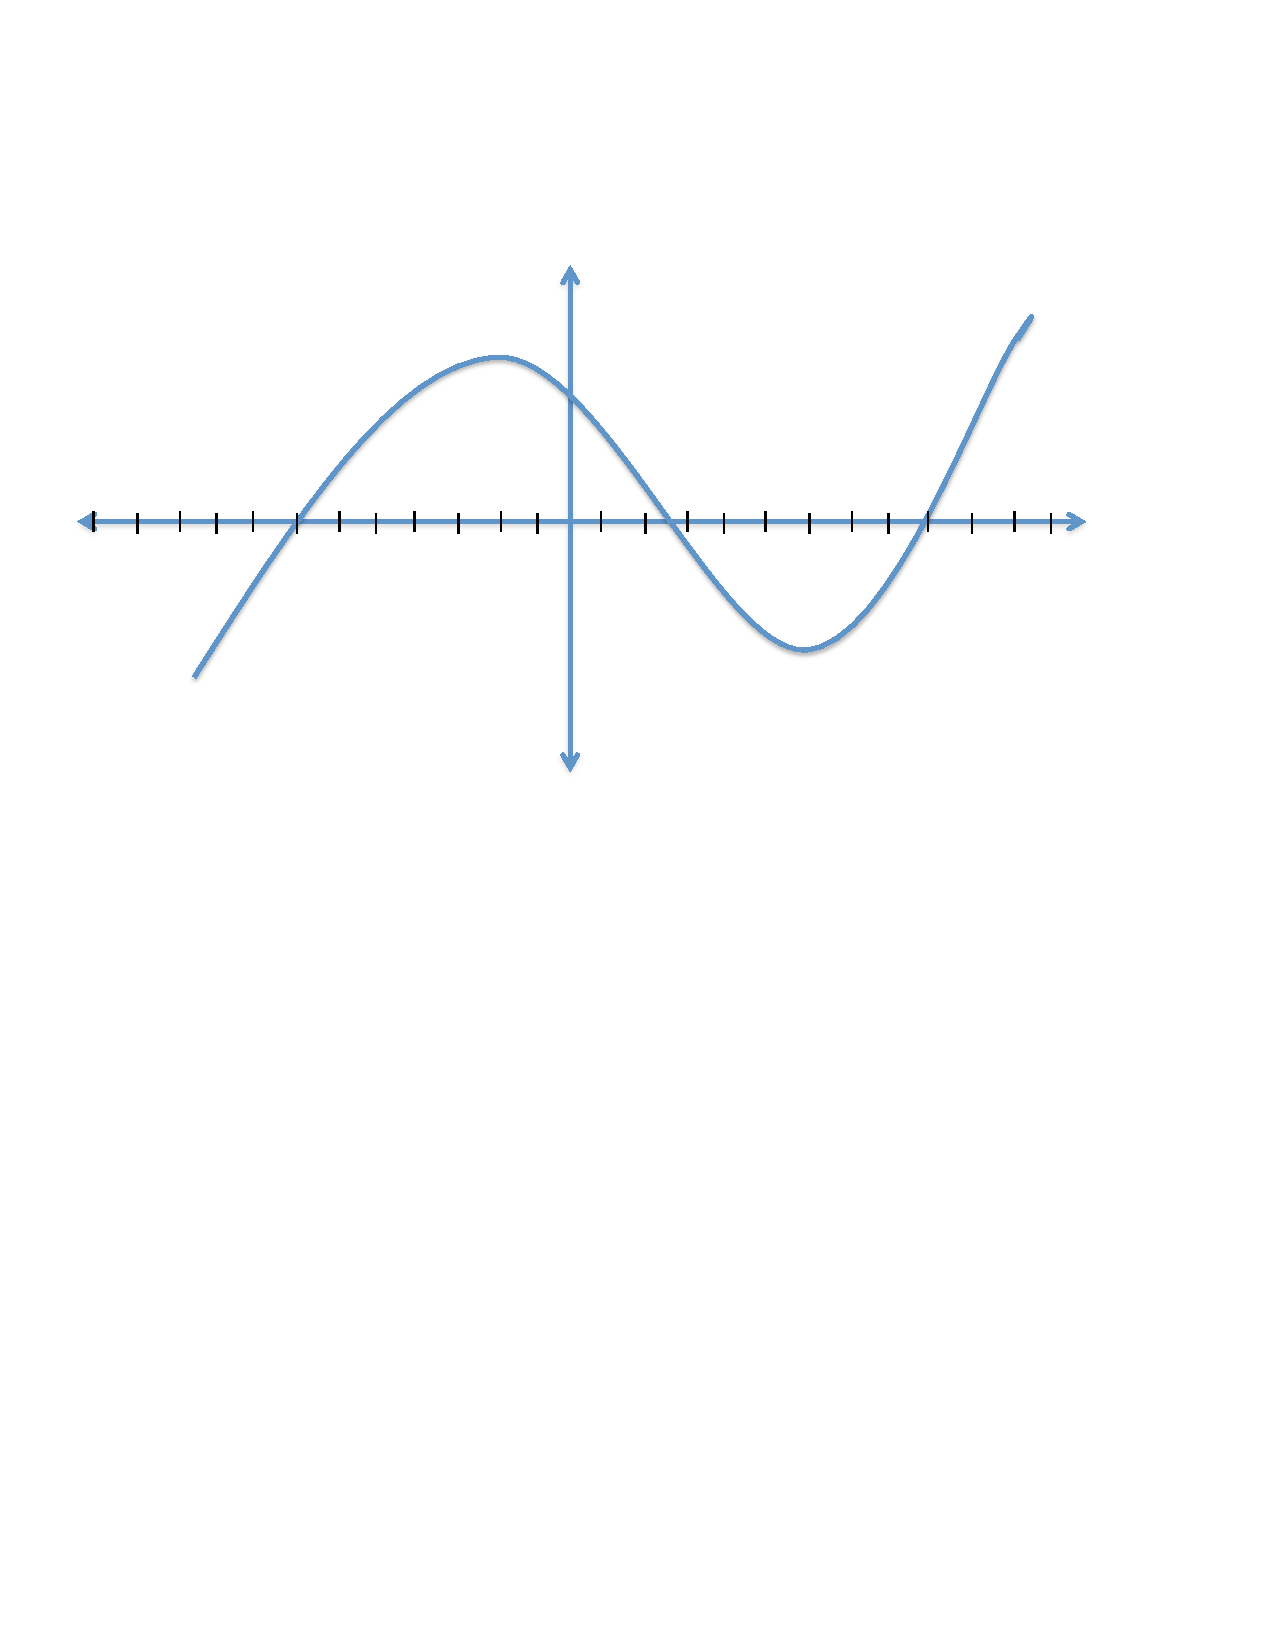
\includegraphics[trim= 170 430 250 100]{Images/Figure2.pdf}
  \end{image}
  \begin{itemize}
    \item[(a)]
      Using this graph find
      \begin{itemize}
        \item 
          all $x$ where $f(x) = 0$,
        \item 
          all $x$ where $f(x) > 0$, 
        \item
          all $x$ where $f(x) < 0$, and
        \item
          all $x$ where $f(x)$ is highest and all $x$ where $f(x)$ is lowest.
      \end{itemize}

    \item[(b)]
      Without sketching the graph of $f'$ find
      \begin{itemize}
        \item 
          all $x$ where $f'(x) = 0$,

        \item
          all $x$ where $f'(x) > 0$,
        
        \item
          all $x$ where $f'(x) < 0$, and

        \item
          all $x$ where $f'(x)$ is highest and all $x$ where $f'(x)$ is lowest.
      \end{itemize}

    \item[(c)]
      Determine where $f$ is the steepest.
      (What does this mean in terms of $f'$?)

    \item[(d)]
      Sketch a graph of $f'$.
  \end{itemize}
\end{problem}

\begin{problem}
  Use the graph of $g$
  \begin{center}
    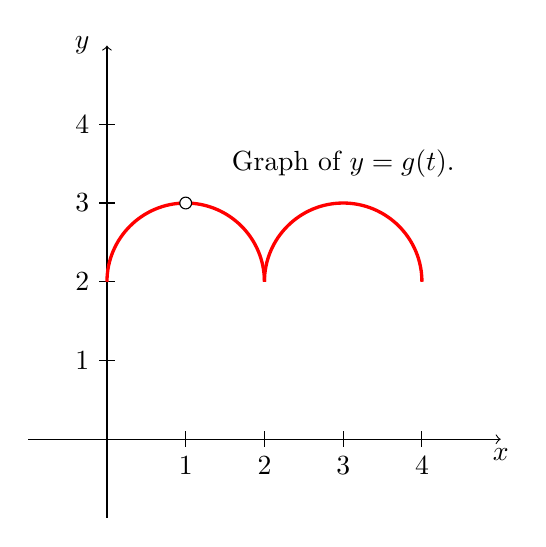
\begin{tikzpicture}
      %\draw[help lines] (-1,-1) grid (5,5);
      \draw [->] (-1,0) -- (5,0);
      \draw [->] (0,-1) -- (0,5);

      \draw (1,0.1) -- (1,-0.1);
      \draw (2,0.1) -- (2,-0.1);
      \draw (3,0.1) -- (3,-0.1);
      \draw (4,0.1) -- (4,-0.1);
      \draw (-0.1,1) -- (0.1,1);
      \draw (-0.1,2) -- (0.1,2);
      \draw (-0.1,3) -- (0.1,3);
      \draw (-0.1,4) -- (0.1,4);

      \draw (1,-0.1)node[below]{$1$};
      \draw (2,-0.1)node[below]{$2$};
      \draw (3,-0.1)node[below]{$3$};
      \draw (4,-0.1)node[below]{$4$};
      \draw (5,0)node[below]{$x$};
      \draw (-0.1,1)node[left]{$1$};
      \draw (-0.1,2)node[left]{$2$};
      \draw (-0.1,3)node[left]{$3$};
      \draw (-0.1,4)node[left]{$4$};
      \draw (-0.1,5)node[left]{$y$};

      \draw (3,3.5)node{Graph of $y = g(t)$.};

      \draw[red, very thick] (2,2) arc [radius=1, start angle=0, end angle = 180];
      \draw[red, very thick] (4,2) arc [radius=1, start angle=0, end angle = 180];

      \draw[fill=white] (1,3) circle [radius=0.075];
    \end{tikzpicture}
  \end{center}
  to find
  \begin{itemize}
    \item[(a)]
      the values of $t$ in $(0, 4)$ where $g$ is \emph{not} continuous, and

    \item[(b)]
      the values of $t$ in $(0, 4)$ where $g$ is \emph{not} differentiable.
  \end{itemize}
\end{problem}

\begin{problem}
  Given the following graph of a function $h$ sketch a graph of the derivative $h'$.
  \begin{image}
% trim= 250 390 250 160
    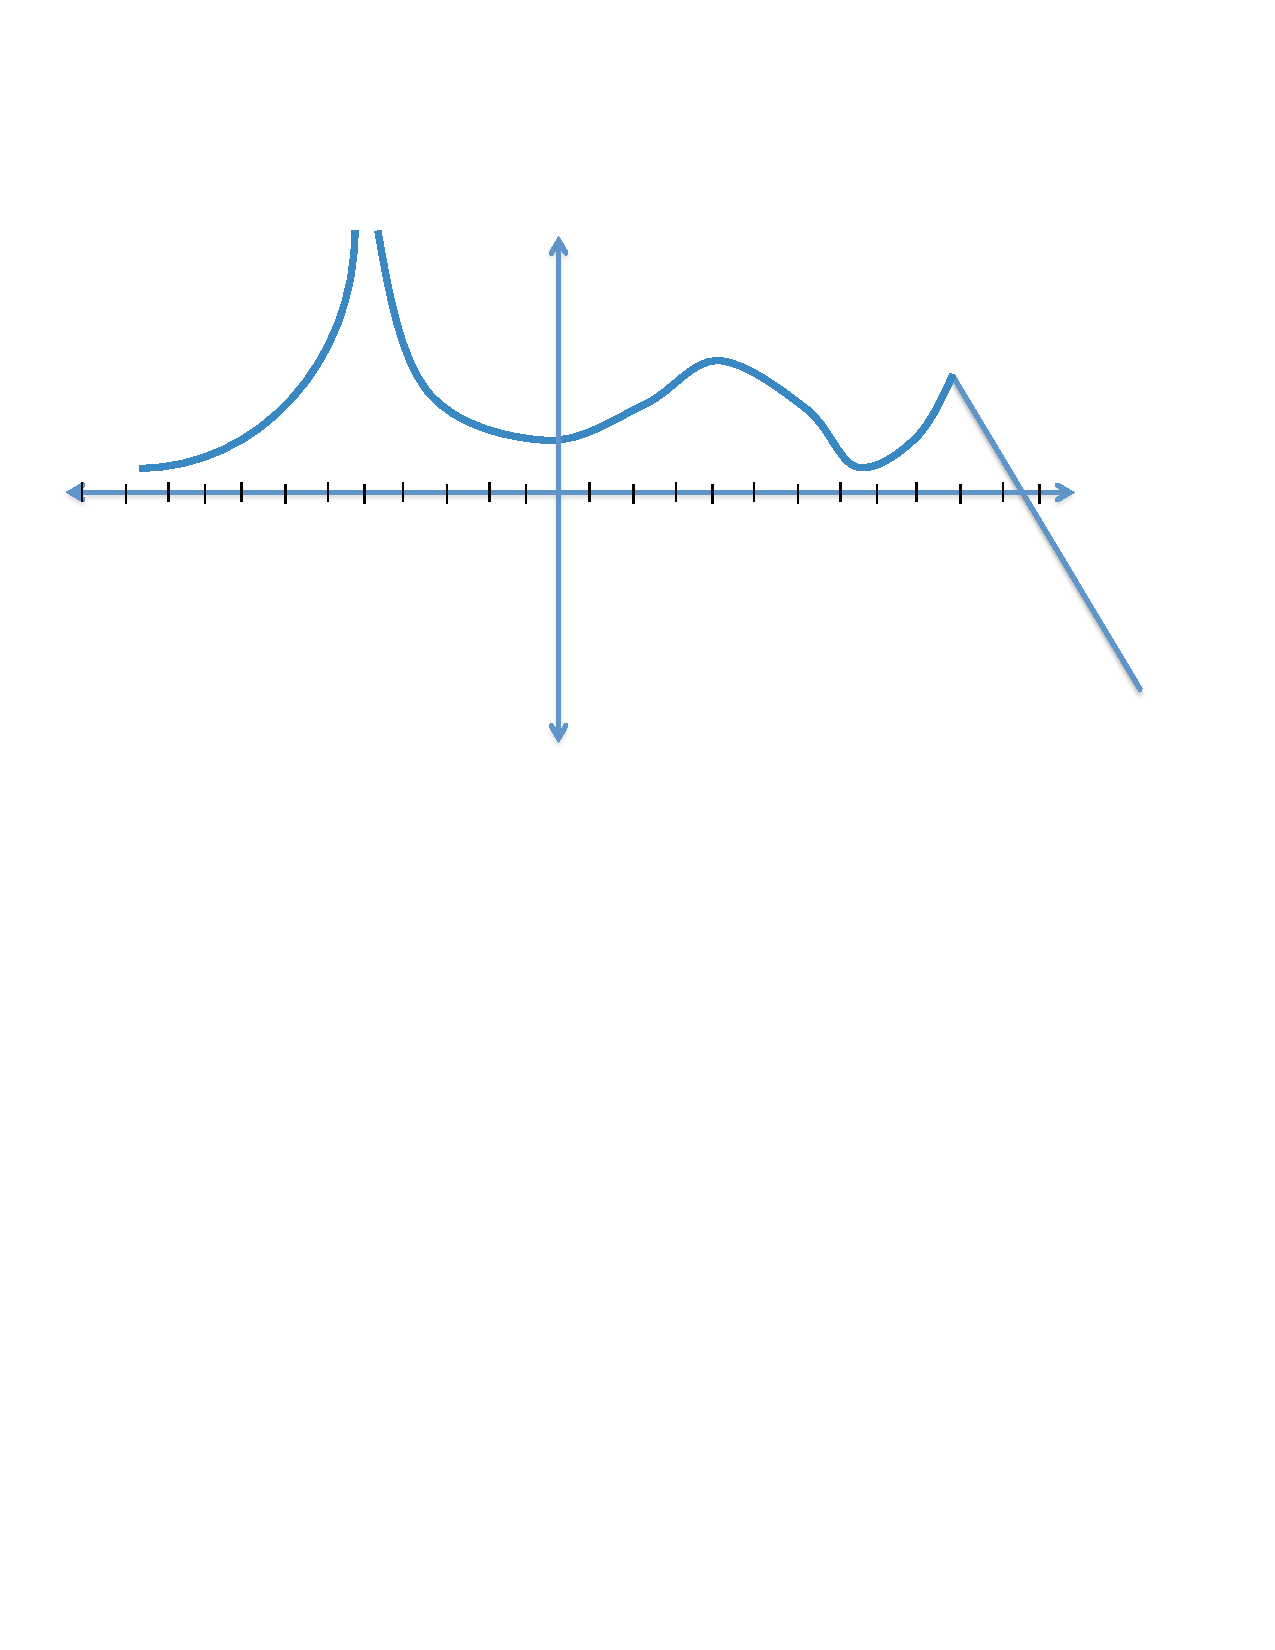
\includegraphics[trim= 170 430 250 100]{Images/Figure5.pdf}
  \end{image}

\end{problem}
\begin{problem}
  \mbox{}
  \begin{itemize}
    \item[(a)]
      Fill in the blanks
      \[
        f'(x) = \lim_{\underline{\hspace{2em}}} \frac{\hspace*{8em}}{h}
      \]
      if the limit exists.

    \item[(b)]
      Let 
      \[
        f(x) = \frac{1}{x + 4}.
      \]
      Use the (limit) \emph{definition} of derivative in (a) to find $f'(x)$.

      \textsc{Do not use the produce or quotient rule! Show your work!}
  \end{itemize}
\end{problem}

\section{Extra problem for personal practice}
\begin{problem}
  The following work shows how we find the derivative of the function $f$ defined by $f(x) = x/(x-5)$ at $x = 3$ using the definition of the derivative:
  \begin{align*}
    f'(3) &= \lim_{h \to 0} \frac{f(3 + h) - f(3)}{h} = \lim_{h \to 0} \frac{\frac{3+h}{(3+h) - 5} - \frac{3}{3-5}}{h}\\
    &= \lim_{h \to 0} \left[\frac{3+h}{(3+h) - 5} - \frac{3}{3-5}\right]\frac{1}{h} \\
    &= \lim_{h \to 0} \left[\frac{(3+h)(3-5)}{[(3+h) - 5](3-5)} - \frac{3[(3+h)-5]}{(3-5)[(3+h)-5]}\right]\frac{1}{h} \\
    &= \lim_{h \to 0} \frac{(3+h)(3-5) - 3[(3+h)-5]}{[(3+h) - 5](3-5)h}\\
    &= \lim_{h \to 0} \frac{3 \cdot 3 + 3\cdot (-5) + 3h - 5h -[3\cdot3 + 3h + 3\cdot(-5)]}{[(3+h) - 5](3-5)h}\\
    &= \lim_{h \to 0} \frac{9 -15 + 3h - 5h -9 - 3h + 15}{[(3+h) - 5](3-5)h}\\
    &= \lim_{h \to 0} \frac{-5h}{[(3+h) - 5](3-5)h} \\
    &= \lim_{h \to 0} \frac{-5}{[(3+h) - 5](3-5)} = \frac{-5}{[(3+0) - 5](3-5)}\\
    &= \frac{-5}{(3-5)^2} = \frac{-5}{4}.
  \end{align*}
  \begin{itemize}
    \item[(a)]
      Adapt this work to find a formula for $f'$.

    \item[(b)]
      What is the domain of $f'$?

    \item[(c)]
      What is the range of $f'$?

    \item[(d)]
      Sketch a graph of $f'$.
  \end{itemize}
\end{problem}
\end{document} 
